\subsection{Bildegjenkjenning}

Vi ble anbefalt å bruke OpenCV av Kongsberg, et open source softwarebibliotek som brukes til bearbeiding av bilder og video. I tillegg til bruken av OpenCV ble vi oppfordret til å bruke Matlab for å programmere. Noen på gruppa hadde erfaringer i Matlab fra før, så vi betraktet ikke dette som noe stort problem.

For å bruke Matlab og OpenCV sammen trengte vi et annet open source prosjekt som het ``mexopencv''. Vi forsøkte en stund å få dette til å fungere, men vi hadde problemer med å sette opp C++, OpenCV og Matlab på en slik måte at mexopencv kunne bruke alle disse ressursene. Noe som førte til ekstra problemer var at de som hadde ansvaret for å begynne med programmeringen satt på to ulike operativsystemer og dermed opplevde forskjellige feilmeldinger underveis. 

Til slutt valgte vi å gå for en løsning hvor vi ikke brukte Matlab. Dette førte til at vi raskt kunne komme igang med utviklingen av bildegjenkjenning og hadde en enkel løsning oppe i løpet av noen dager.

\subsubsection{Første steg}

Den første implementasjonen av gjenkjenningen baserte seg på å konvertere en frame av videoen fra det normale fargespekteret RGB, se figur [\ref{fig:firstiterationrgb}], til et fargespektrum som het HSV\footnote{Hue, Saturation and Value} som vist i figur [\ref{fig:firstiterationhsv}].

\begin{figure}[h!]
	\centering
	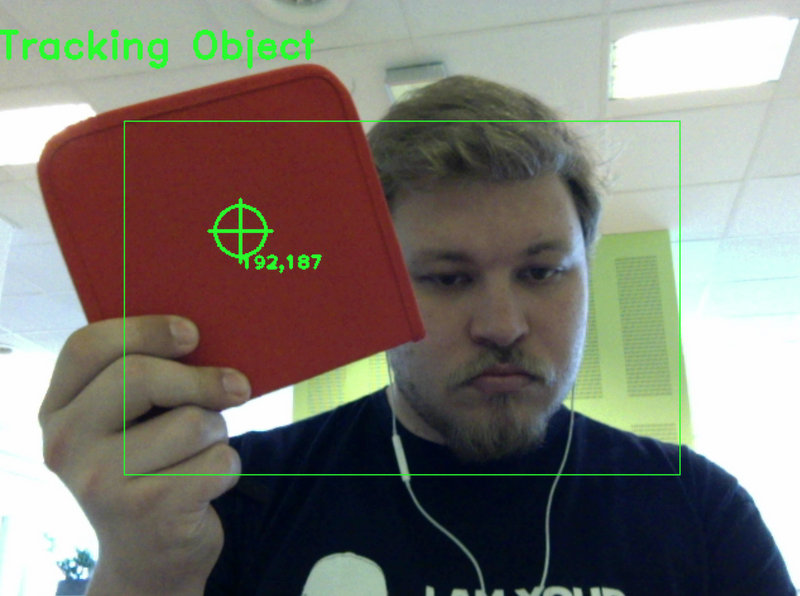
\includegraphics[scale=0.45]{img/first-rgb.jpg}
	\caption[Første iterasjon RGB bilde]{Bilde fra video i vanlig RGB}
	\label{fig:firstiterationrgb}
\end{figure}

\begin{figure}[h!]
	\centering
	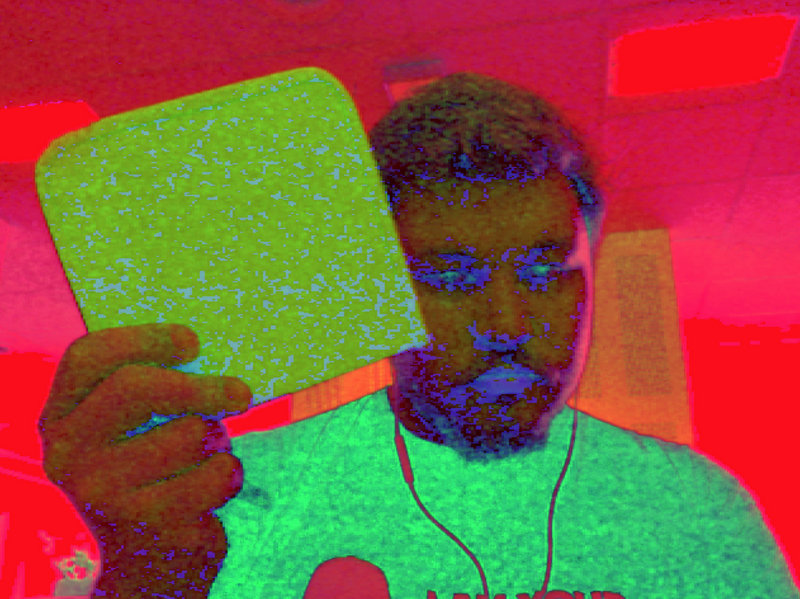
\includegraphics[scale=0.45]{img/first-hsv.jpg}
	\caption[Første iterasjon HSV bilde]{Bilde fra video oversatt til HSV}
	\label{fig:firstiterationhsv}
\end{figure}

HSV baserer seg ikke på blandingen av farger, men bruker nyanser, metningsgrad og lysverdier for å vise en farge . Matrisen med fargekoder som skapes av konverteringen til HSV fører til en skarpere kontrast mellom farger, og gjør jobben med å filtrere vekk uønskede elementer lettere. Vi behandlet deretter matrisen med et filter, som vi manuelt stilte inn med maksimum- og minimumverdier for henholdsvis Hue, Saturation og Value, vist i figur [\ref{fig:sliders}]. Etter at matrisen hadde passert gjennom filteret satt vi igjen med et binært bilde, der fargene som passerte gjennom filteret er gjengitt som hvitt, mens alle andre farger er svarte slik det er vist i figur [\ref{fig:firstiterationbinary}].

\begin{figure}[h!]
	\centering
	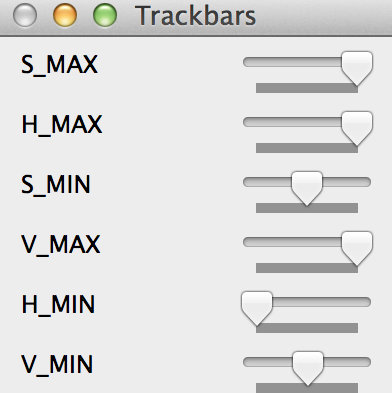
\includegraphics[scale=0.45]{img/sliders.jpg}
	\caption[First iteration HSV image]{Frame from video cast to HSV}
	\caption{Slidere for å velge HSV verdier}
	\label{fig:sliders}
\end{figure}

\begin{figure}[h!]
	\centering
	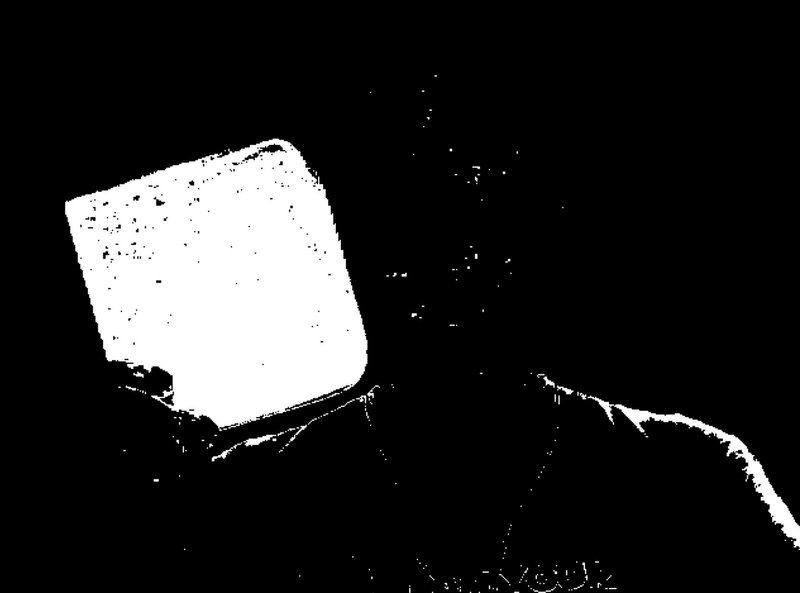
\includegraphics[scale=0.45]{img/first-binary.jpg}
	\caption[Første iterasjon binært bilde]{Resultatet av filtrering av et HSV bilde før smoothing}
	\label{fig:firstiterationbinary}
\end{figure}

\subsubsection{Andre steg}

I det første steget klarte vi å fange opp et objekt, men som man kan se i figur [\ref{fig:firstiterationbinary}] er det mye støy i bildet. Vi implementerte derfor en smoothingalgoritme som gikk over det binære bildet og fjernet mindre ansamlinger med punkter og fremhevet de som var større. Dette førte til at vi fikk et renere bilde, med færre og tydeligere objekter. Dette gjorde det betydelig lettere å fange opp de enkelte objektene i bildet og finne det største av dem.

Resultatet kan man se i figur [\ref{fig:seconditerationbinary}] 

\begin{figure}[h!]
	\centering
	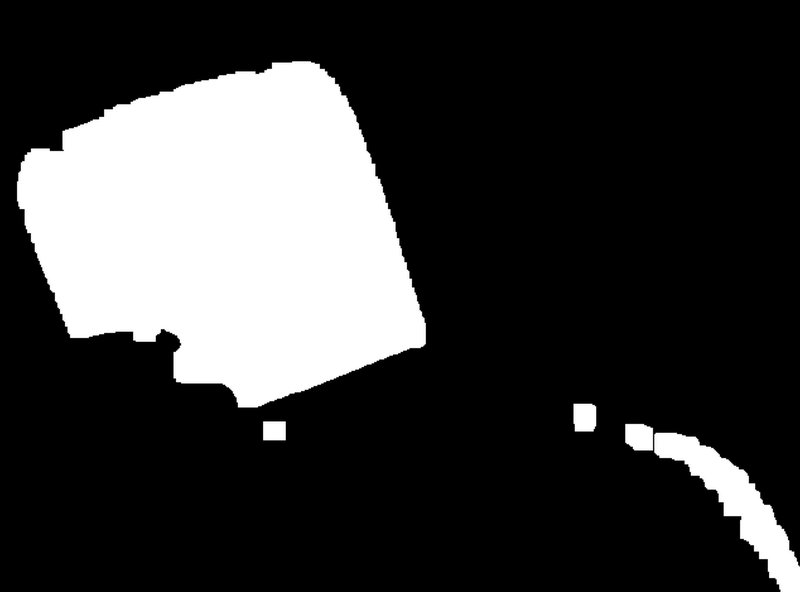
\includegraphics[scale=0.45]{img/second-binary.jpg}
	\caption[Andre iterasjon binært bilde]{Resultatet av filtrering av et HSV bilde etter smoothing}
	\label{fig:seconditerationbinary}
\end{figure}

\subsubsection{Tredje steg}

Etter at vi hadde jobbet en del med systemet fant vi ut at det var tungvindt å stille inn verdiene som skulle følges hver gang. Løsningen ble da at vi implementerte et enkelt kommandogrensesnitt som kunne be programmet om å følge etter fargen som befant seg i sentrum av bildet, som vist i figur [\ref{fig:commandmenu}]

\begin{figure}[h!]
	\centering
	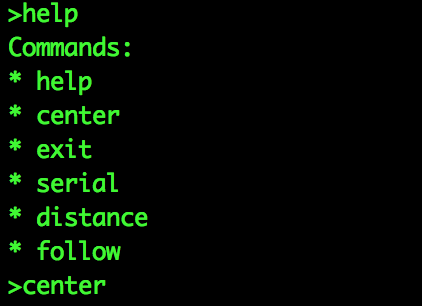
\includegraphics[scale=0.8]{img/command-menu.png}
	\caption{Kommandomenyen}
	\label{fig:commandmenu}
\end{figure}

\subsection{Konstruksjon av riggen}

\subsubsection{Planlegging}
Riggens oppgave er å endre synsretningen til kameraet etter kommando fra bildegjennkjenningen. Synsvinkelen kan modeleres som en vektor, hvor retningen til vektoren er variabel. Hvis vektoren, $\bf{v}$, settes inn i et koordinatsystem med utspring i origo og sfæriske koordinater, kan situasjonen beskrives som i figur [\ref{fig:spher}]

\begin{figure}[h!]
	\centering
	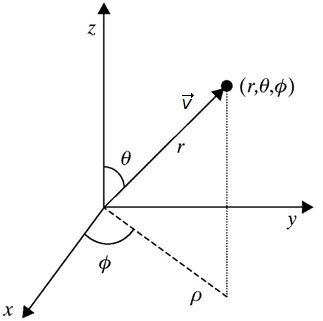
\includegraphics[scale=0.5]{img/RettVek.jpg}
	\caption{Sfærisk koordinatsystem}
	\label{fig:spher}
\end{figure}

hvor $\phi$ er vinkelen mellom x- og y-aksene og $\theta$ er vinkelen mellom z-aksen og xy-planet. Siden riggen skal festes til et fly og kameraet skal se ned på bakken vil det ikke være behov for vinkelretningen å bevege seg inn i den øvre halvdelen av koordinatsystemet. Det betyr at $\phi$ og $\theta$ kun trenger 180 graders utsving for å dekke hele den nedre halvdelen. Dermed kan hele dette omerådet dekkes ved hjelp av to servomotorer med 180 graders utslag satt sammen som i figur [\ref{fig:IdeRigg}]. 

\begin{figure}[h!]
	\centering
	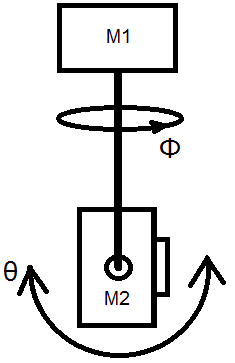
\includegraphics[scale=0.5]{img/BasicRiggIde.png}
	\caption{Servostyring av $\theta$ og $\phi$}
	\label{fig:IdeRigg}
\end{figure}

Hvor kameraet festes til servomotor 2 som beveger seg i retning $\theta$, mens servomotor 1 beverger servo2 og kamera i retning $\phi$. For å kunne trekke riggen inn i flyet ved landing ble det bestemt å feste riggen på en bom som kunne heves å senkes ved hjelp av en servomotor som vist i figur [\ref{fig:bom}].

\begin{figure}[h!]
	\centering
	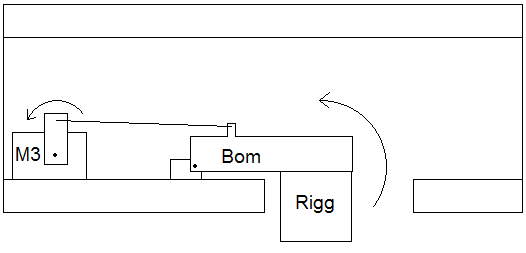
\includegraphics[scale=0.5]{img/Motor3.png}
	\caption{Servomotor 3 kan heve riggen inn i flykroppen.}
	\label{fig:bom}
\end{figure}


\subsubsection{Sammenstilling}
Riggen ble sammenstilt med målene på prototypeflyet til kongsberg som utgangspunkt [\ref{ref:PowerPoint}]. Med disse målene ble det klart at servomotorene måtte være små i størrelse og valget falt på servomotoren HD-1600A. Med sine beskjedene fysiske mål på 21.3x11.6x22.8 mm og en vekt på 6g [\ref{ref:PowerHD}], ble HD-1600A ansett som perfekt for dette formålet. HS-50 fra Hitec ble også vurdert, men med lavere dreimoment og betydelig høyere pris ble HD-1600A regnet som et bedre alternativ. For å bygge delene som skulle koble servoene sammen ble det brukt 6mm MDF plater fordi disse er stive og relativt sterke. Dette fører til at de ikke bøyes eller gir etter ved raske rotasjoner. Figur [\ref{fig:RiggTegn}] viser hvordan servomotorene er koblet sammen og figur [\ref{fig:RiggBilde}] viser et bilde av den ferdige prototype riggen. 

\begin{figure}[h!]
	\centering
	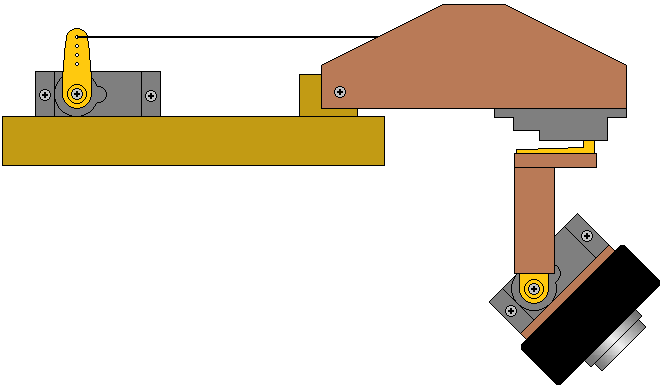
\includegraphics[scale=0.5]{img/RIGG_sattsammen.png}
	\caption{Tegning av mekaniske rigg}
	\label{fig:RiggTegn}
\end{figure}

Servomotorene styres av et PWM signal som genereres av en Arduino UNO. Biblioteket $Servo.lib$ brukes for å kontrollere servoene gjennom tre I/O porter. Servo 1 er koblet til port 9, servo 2 er koblet til port 6 og servo 3 er koblet til port 3. Siden det viste seg ved målinger at hver servo, under last, kan trekke opp mot 250mA, ble det valgt å bruke en ekstern 6V batteripakke, med fire seriekoblede 1.5V AA batterier, koblet inn som vist i figur [\ref{fig:ArduSkjem}]. Dette isteden for å la servoene trekke forsyningsstrøm rett fra 5V pinnen til arduinokortet. Arduinokortet bruker strøm fra USB og denne kan ikke levere mer enn 500mA ,på grunn av innebygget sikring i Arduino. Dermed kan ikke Arduinokortet levere de ca. 750mA som trengs dersom alle servoene går med stor last samtidig. 

\begin{figure}[h!]
	\centering
	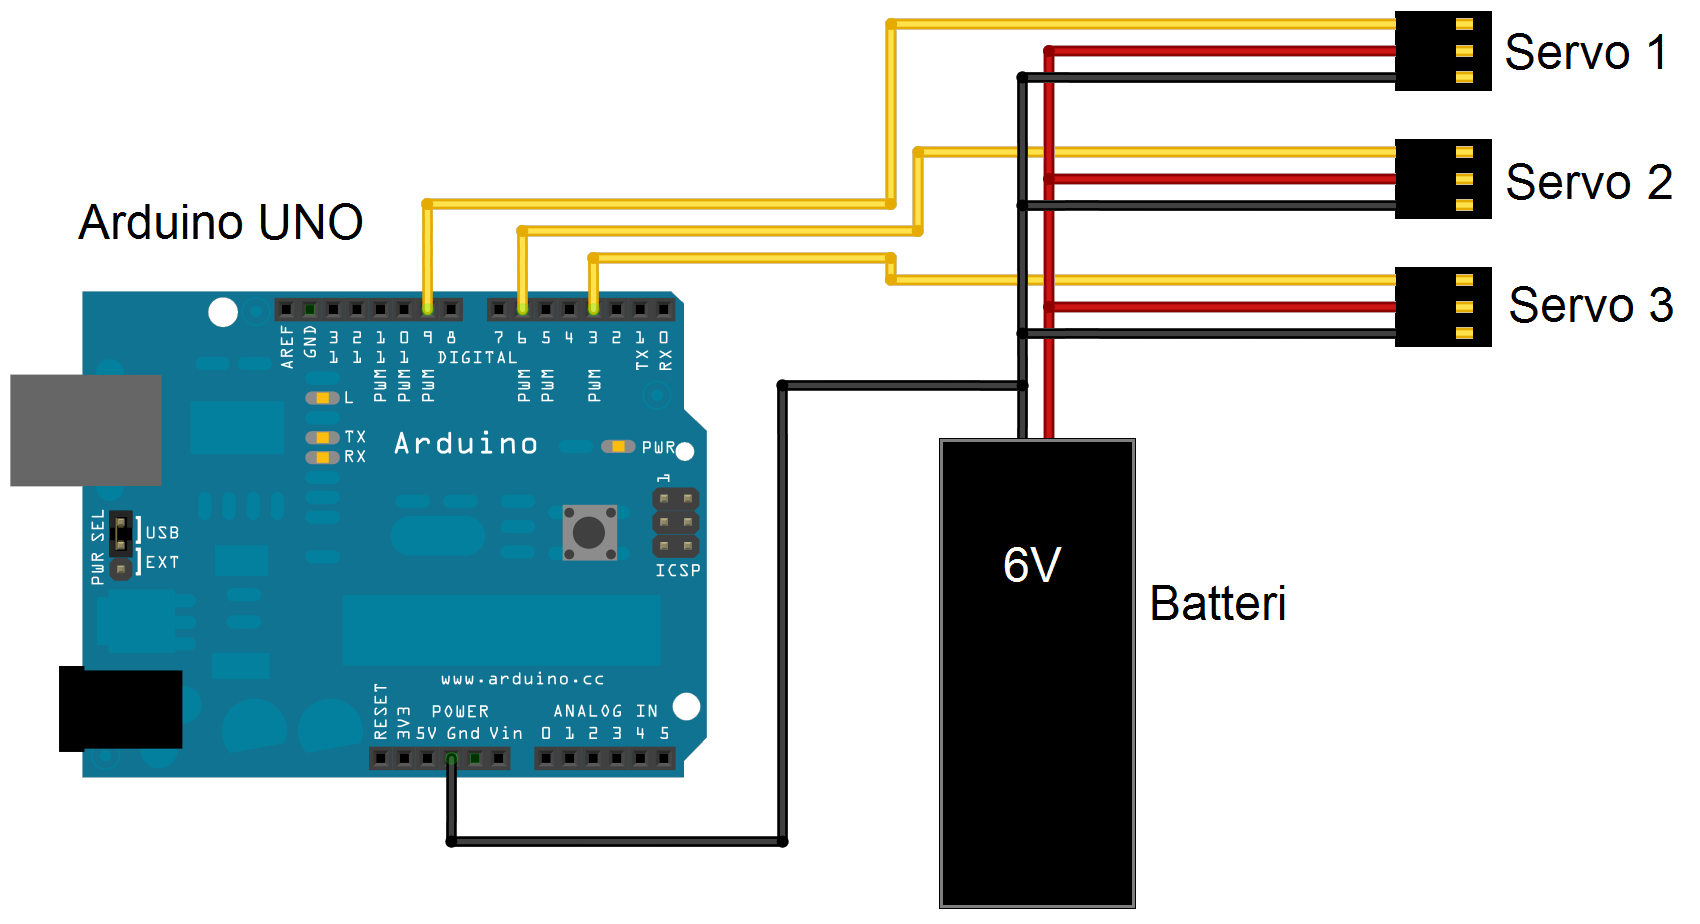
\includegraphics[scale=0.25]{img/KoblingsskjemaArduino.png}
	\caption{Koblingsskjema for Arduino}
	\label{fig:ArduSkjem}
\end{figure}  

Kommandoer sendes til Arduino via USB porten. Kommandoer kan sendes som $Char$ på formen ``100a120b40c'', hvor tallene foran``c'' forteller posisjon til servo 1, tallene for ``b'' gir posisjon til servo 2 og tallene foran ``c'' posisjonenen til servo 3. Dermed vil strengen ``100a120b40c'' flytte servo 1 til 100 grader, servo 2 til 120 grader og servo 3 til 40 grader. De gyldige vinklene er fra 0 til 180 grader. Hvis ``200'' sendes vil servo 1 stoppe på 180 grader. 


\subsection{Styring av rigg + bildegjenkjenning}

Tekst her